\section{Macro implications of perceived job risks}

\subsection{Shocks or risks?}

In the previous sections, with the three measures in hand, namely (a) perceived risks, $\widehat{JF}$/$\widetilde{JS}$, (b) objective risks $\widehat{JF}^*$/$\widehat {JS}^*$, and (c) realization of job flow rates $JF$/$JS$, we have established two major findings. The first is a rejection of perfect foresight, in that even ex-ante rational and fully informed forecasts of risks don't fully predict ex-post realizations.  This is indicated by the gap between (b) and (c). The second is the deviation of ex-ante perceived job risks from its true ex-ante counterpart, at least partially due to information rigidity.  

But do the distinctions between (a), (b), and (c) matter for aggregate fluctuations? We can assess empirically the relative importance of ex-ante precautionary saving motives resulting from perceived job risks (a), responses due to misperceived risk ((a)- (b)), and ex-post responses due to truly unexpected income shocks ((b)-(c)), by comparing the cyclical properties of (a), (b) and (c) across business cycles. 

We use two sets of metrics to evaluate the relative importance of the three channels. The first one is the unconditional standard deviation of (a), (b), and (c). The second metric is the ratio between the onset and the end of each recession in our sample. More intuitively, they reflect the changes in these rates from the peak to the trough of each cycle. 

Throughout our data sample 1990-2024 which covered four recessions and experienced sizable cyclical movements of unemployment risks, the unconditional standard deviation of realized job-finding rates is approximately 7.2 percentage points. Most of these variations are reflected in real-time finding probabilities, whose standard deviation was about 6.9 percentage points. In contrast to these cyclical movements of realized job finding rates, the perceived finding rates exhibit milder fluctuations and have a standard deviation of 4 percentage points. In the domain of job separation, the unconditional standard deviations of perceptions, risk forecast, and realizations are 1.0, 0.9, and 0.3 percentage points, respectively. Both finding and separation perceptions move significantly less than the realized job risks. 

Such rankings of the relative volatility of perceptions and realizations also can be seen in Figure \ref{fig:bus_cycle_stats} which reports the peak and trough rates in each of the four recessions in the sample period. From the onset of each recession to its end month, the real-time job finding drops by 25\%, while the perceptions of job finding only decrease by 15\%. 

Meanwhile, average job separation perceptions are much more sluggish than job finding expectations, which is again confirmed by on average a 16\% increase from the start to the end of each recession, as opposed to a 50\% average increase in job separation risk forecast and 150\% in realized job separation rates. The increase in realized job separation rates remains high with the pandemic recession excluded, which was not reflected in the change in perceptions.  

\begin{figure}[pt] 
\centering 
	\caption{Business Cycle Patterns of Risks and Perceptions: Start versus End of Recessions} 
	\label{fig:bus_cycle_stats}
\includegraphics[width=0.99\linewidth]{text/chapter2/Figures/business_cycle_JF_peak_trough.pdf} \\
\includegraphics[width=0.99\linewidth]{text/chapter2/Figures/business_cycle_JS_peak_trough.pdf} \\
 	
    	\begin{flushleft}\footnotesize {Note: The left tables report the perceived job risks, perceived job risks at different quantiles, real-time job risks, and realized job transition rates at the beginning and the end month of each one of the four recessions. The bar chart on the right plots the peak-to-trough ratios of these rates. The sample period is 1990-2024.} \end{flushleft}
\end{figure}

Such average patterns mask substantial heterogeneity in job risks and perceptions. Figure \ref{fig:bus_cycle_stats} also plots the movements of perceptions over business cycles by agents at different percentiles of perceived job risks. In terms of job-finding, although an average worker's perceived job finding probability drops by 15\% from the peak to trough of a recession, more or less comparable to the realized job finding, it is the low-finding rate worker, at 25 percentile who perceive a much sharper drop by about 25\%, compared to a drop of 10\% for the worker at the 75th percentile. In terms of job separation, although an average worker's job loss perceptions only increase by 15 percentage points in recessions, the \emph{median} worker's perceptions increased much more sharply by about 35 percentage points. Recessions hit agents in the economy unevenly in terms of their job risks. Such heterogeneity in perceptions reveals the uneven footprints of business cycle fluctuations via job risk changes. Heterogeneity in risk exposure implies different degrees of ex-ante precautionary saving behaviors and their consequent ex-post shock responses, a topic we turn to in the next section. 


%Using perceived risk and realized flow rates, we can also construct true unexpected shocks to job risks in business cycles and see their effects on consumption spending. 

%Our estimated heterogeneity in job risks the distribution of $\eta_{i,t}$ and the average information rigidity $\lambda$ for each group can be used to calibrate HANK models featuring belief distortions and heterogeneous job risks.

\subsection{Quantifying the aggregate consumption impacts of unemployment risks}


In this section, we show that the strength of the unemployment risk channel changes substantially when household beliefs are instead disciplined by survey data on workers’ expectations of finding and losing a job instead of the realized counterparts of these probabilities. Furthermore, we demonstrate that the magnitude of this channel differs significantly across education groups.

To assess the extent to which consumption fluctuations are driven by precautionary behavior versus realized income losses from unemployment, we simulate the path of aggregate consumption dynamics by feeding our time series of perceived and objective unemployment risk, and our measures of observed (un)employment transition rates into a standard heterogeneous agent model with persistent unemployment.

 The model is set to a monthly frequency. In the model, workers make a consumption-saving decision in the face of both idiosyncratic productivity shocks and stochastic transition between employment and unemployment. Transitions between (un)employment states are dictated by the job separation and job finding probability. Workers’ perceptions of job finding and separation probabilities are distinct states, separate from the probabilities that govern their actual transitions between employment and unemployment. Self-insurance is achieved by saving money on a risk-free asset. Finally, during unemployment, households receive unemployment insurance. Figure \ref{fig:model_timeline} illustrates the timeline of the model. Details of the model specifications are found in Appendix \ref{appendix:model}. The calibration of the model can be found in table \ref{table:Calibration}.


\subsubsection*{Decomposition of consumption Jacobians}


 We first decompose the sequence space consumption Jacobians—following the approach of \cite{auclert2021using}-with respect to job separation probability into a precautionary effect and an income effect stemming from changes in unemployment to highlight that a greater degree of aggregate precautionary saving dampens the income effect. Furthermore, we utilize these decomposed jacobians to simulate the path of aggregate consumption under different counterfactual. 
 
Figure~\ref{fig:jac_decompose} illustrates the consumption response to an increase in the job separation probability at horizon \( t + h \), with \( h = 10 \). The black line corresponds exactly to the 10\textsuperscript{th} column of the consumption Jacobian with respect to the job separation probability. The \textit{ex-ante} component captures the anticipatory behavior reflected in the black line---that is, the self-insurance response of workers leading up to the increase in separation risk at \( t = 10 \), under the assumption that the risk itself does not actually materialize. In contrast, the \textit{ex-post Jacobian} captures the consumption response to the realized increase in unemployment resulting from an actual rise in the separation probability, assuming workers do not anticipate this change.



\begin{figure}[pt]
    \centering
    \caption{Timeline of the Model}
    \label{fig:model_timeline}
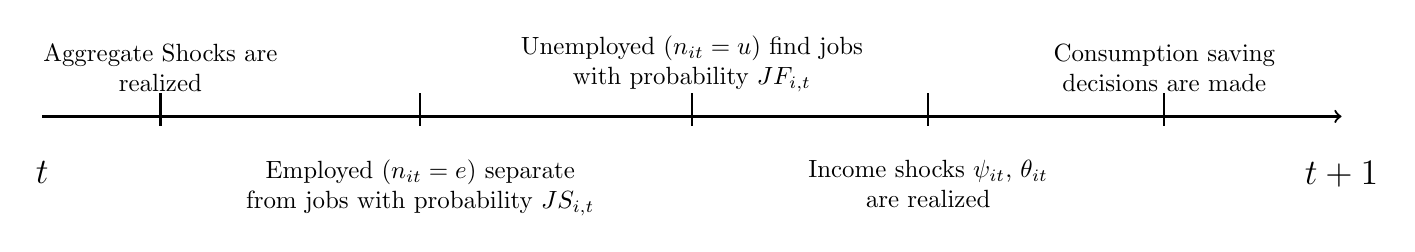
\begin{tikzpicture}[thick,scale=1.5, every node/.style={scale=.9}]
  % Set the timeline's limits
  \draw[->] (0,0) -- (11,0);
  \draw (11,-.3) node[below] {\Large $t+1$};
  \draw (0,-.3) node[below] {\Large $t$};
  % Add events
  \draw (1.,-.08) node[above=10pt,align=center] {Aggregate Shocks are\\realized} -- (1.,0.2);
  \draw (3.2,-.08) node[below=10pt,align=center] {Employed ($n_{it}=e$) separate\\from jobs with probability $JS_{i,t}$} -- (3.2,.2);
  \draw (5.5,-.08) node[above=10pt,align=center] {Unemployed ($n_{it}=u$)  find jobs\\with probability $JF_{i,t}$} -- (5.5,0.2);
  \draw (7.5,-.08) node[below=10pt,align=center] {Income shocks $\psi_{it}$, $\theta_{it}$ \\are realized} -- (7.5,0.2);
  \draw (9.5,-.08) node[above=10pt,align=center] {Consumption saving\\decisions are made} -- (9.5,0.2);

\end{tikzpicture}
\end{figure}



Figure~\ref{fig:jac_decompose_sub} illustrates how underreactive beliefs---as documented in survey expectations about both job finding and job loss probabilities---weaken the precautionary channel while amplifying the income loss channel associated with unemployment. The figure includes two additional consumption responses under the assumption of sticky belief updating. The purple line shows the \textit{subjective} consumption response to an increase in the job separation probability at \( t = 10 \), assuming that in each period from \( t = 10 \) onward, 10\% of workers update their expectations. The red line shows the same response with the additional assumption that the job separation probability never effectively increases. The \textit{ex-ante} component of the response is significantly muted relative to the full (objective) response shown in black. However, the consumption drop at \( t = 10 \) and beyond is substantially larger, reflecting a lack of precautionary saving and thus a lack of self-insurance.

\begin{figure}[pt]
    \centering
    \caption{Consumption Jacobian to an anticipated 10-period-ahead shock to the job separation}
    \label{fig:jac_decompose}
%\includegraphics[width=0.9\textwidth]{Figures/JF_decomposition.pdf} 
\includegraphics[width=0.8\textwidth]{text/chapter2/Figures/JS_decomposition.pdf} 
\floatfoot{\footnotesize{This figure plots the total and decomposed Jacobians of the aggregate consumption with respect to an anticipated shock to job separation probability at $t+10$. The Jacobian is defined exactly as in \cite{auclert2021using}. }}
\end{figure}


\begin{figure}[pt]
    \centering
    \caption{Subjective Consumption Jacobians with Sticky Expectations}
    \label{fig:jac_decompose_sub}
%\includegraphics[width=0.8\textwidth]{Figures/JF_decomposition_subjective.pdf} \\
\includegraphics[width=0.8\textwidth]{text/chapter2/Figures/JS_decomposition_subjective.pdf} 
\begin{flushleft}\footnotesize {Note: The figure shows the aggregate consumption Jacobian concerning a future shock to job-separation rate that is broken down into those driven by ex-ante perceived risk and that is caused by ex-post shock response in full-information versus subjective/sticky perceptions of job separation risk.} \end{flushleft}
\end{figure}


\subsubsection*{Quantification of consumption impacts}



With the decomposed Jacobians, we simulate of the path of aggregate consumption from 1988 to 2020. Specifically, we estimate AR(1) processes for both our survey-based expectations and the constructed rational expectations of job separation and job finding probabilities, and recover the corresponding shocks that replicate their observed paths from 1988 to 2020. We apply the same procedure to the realized job finding and job separating probabilities estimated from the CPS. These shocks are then fed into the model: household perceptions evolve according to the respective expectation shock series, while actual job transition rates follow the shocks estimated from realized data. This approach generates a simulated path of aggregate consumption that reflects the assumptions underlying each scenario.

We conduct this simulation under four different scenarios. The first assumes that workers do not perceive changes to the job finding and job separation probabilities are only subject to realized changes to the unemployment rate. This simulation isolates the income loss channel of consumption induced from an increase in the unemployment rate. The second assumes that workers' expectations follow our survey based measure of job finding and job loss expectations. The third assumes that workers expectations follow our constructed measure of rational expectations. Finally, the fourth simulation assumes workers have perfect foresight and perfectly anticipate the actual shocks to the job transition probabilities.

Figure~\ref{fig:pe_decompose_sub_obj} shows simulated paths of aggregate consumption from the 1980s through 2020. The two panels isolate the effects of fluctuations in the job separation and job finding probabilities, respectively. Figure ~\ref{fig:pe_decompose_sub_obj_combined} presents the combined effect of both the job finding probability and job separation probability on aggregate consumption. 

Three key findings emerge from the figure. First, when considering job separation alone, the stickiness in separation beliefs leads to a minimal ex-ante precautionary saving response during recessions. Consequently, the total consumption response based on subjective perceptions closely mirrors the ex-post impact and falls short of the response implied by objective risk. Finally, as workers engage in a substantially smaller magnitude of precautionary saving, the recovery of consumption exhibits a more sluggish recovery under subjective beliefs.

Second, in the case of job-finding risk, precautionary saving plays a non-trivial role in driving consumption. However, because beliefs on job finding adjust only partially to the true underlying risk, there is a large a gap between the simulation with objective risk or perfect foresight versus subjective expectations. In the Great Recession, the objective response implies an even larger drop---roughly 1 percentage point more---than the subjective estimate. Just as sluggish job separation beliefs induce a slower recovery, the slow adjustment in job-finding beliefs also contributes to a delayed recovery in aggregate consumption.

Third, the combined impact of job separation and job finding in figure ~\ref{fig:pe_decompose_sub_obj_combined}  is largely driven by the job-finding channel. This reflects two main factors. First, consistent with \cite{fujita2009cyclicality} and the broader search and matching literature, fluctuations in job finding account for a larger share of unemployment dynamics over the business cycle, though the precise contribution is debated. For instance, \cite{broer2021unemployment} argue that job separations shape the short-term response, while job finding drives longer-term dynamics. Second, in our model, job finding risk matters not only for the unemployed but also for the employed, as workers face the possibility of job loss followed by difficulty finding re-employment.  Importantly, beliefs about job finding are also more responsive than those about separation, amplifying the precautionary saving motive. Since our model focuses on non-durable consumption, these estimates likely represent a lower bound. As noted by \cite{carroll1997unemployment} and \cite{harmenberg2021consumption}, the impact of unemployment risk on durable goods consumption is considerably larger.

\begin{figure}[ht]
    \centering
    \caption{Consumption fluctuations due to changes in the job finding probability and to changes in the job separation probability}
    \label{fig:pe_decompose_sub_obj}
\includegraphics[width=0.87\linewidth]{text/chapter2/Figures/consumption_pe_JS_deviation_machine_as_rational_monthly.pdf} \\
\vspace{-2em}
\includegraphics[width=0.87\linewidth]{text/chapter2/Figures/consumption_pe_JF_deviation_machine_as_rational_monthly.pdf} \\
\vspace{-2em}
%\includegraphics[width=0.63\linewidth]{text/chapter2/Figures/consumption_pe_JS_JF_deviation_machine_as_rational_monthly.pdf} \\
	\begin{flushleft}\footnotesize {Note: The figure compares the partial-equilibrium aggregate consumption deviations from its steady state simulated based on empirically estimated shocks to perceived job risk (subjective) and the real-time forecast risk (objective), in addition to the ex-post response to shocks to the realized job transition rates.} \end{flushleft}
\end{figure}


\begin{figure}[ht]
    \centering
    \caption{Consumption Fluctuations due to Unemployment Risks}
        \label{fig:pe_decompose_sub_obj_combined}
\includegraphics[width=1.05\linewidth]{text/chapter2/Figures/consumption_pe_JS_JF_deviation_machine_as_rational_monthly.pdf} \\
	\begin{flushleft}\footnotesize {Note: The figure compares the partial-equilibrium aggregate consumption deviations from its steady state simulated based on empirically estimated shocks to perceived job risk (subjective) and the real-time forecast risk (objective), in addition to the ex-post response to shocks to the realized job transition rates.} \end{flushleft}
\end{figure}
\textbf{Allowing for heterogeneous risks and beliefs} 


Figure \ref{fig:pe_decompose_sub_obj_educ} simulates consumption fluctuations for each education group separately, under the alternative assumption that job risks vary ex-ante by education level. This assumption is motivated by the findings in Section \ref{subsec:hetero_beliefs}, which show that lower-education groups are slower to adjust their perceptions of separation risk, despite facing larger fluctuations in those risks. In contrast, it is the middle-education group whose beliefs about job finding are the most sluggish in responding to real-time changes. We quantify the role of both misperceived risks and overall precautionary saving motives for each group. We calibrate the discount factors for the low- and middle-education groups to target a quarterly marginal propensity to consume (MPC) of 0.34, and for the high-education group to 0.27--values consistent with the estimates reported by \cite{Fuster2020} for individuals without and with a bachelor’s degree, respectively.


We make two findings. First, as expected, the low-education group exhibits the largest ex-post consumption response during recessions, reflecting the interaction between the higher volatility of their realized job transitions and their higher MPC. Second, the high-education group shows a stronger precautionary response overall, driven by their greater sensitivity in updating beliefs. This is evidenced by a smaller gap between their subjective and objective responses, and a larger gap between their subjective and ex-post responses.
Our group-specific anatomy bears aggregate implications. To the extent that the most cyclically exposed groups in job risks are also the ones that have the least sensitivity in reacting to their beliefs and carrying out self-insurance behaviors, which means a larger cut in spending at the moments of the shock, this introduces a potentially important amplification mechanism in the aggregate consumption that is not via its counter-cyclicality per se, but via its heterogeneous footprints. Although heterogeneous risk exposures do not, in general necessarily amplify job risks' impacts on aggregate consumption, they could do so when the heterogeneous workers' risk exposures are positively correlated with their degree of underinsurance. Our results seem to suggest this mechanism is empirically feasible, particularly because workers facing more cyclical risks tend to underreact to such movements in job risks. 

Our group-specific analysis has important aggregate implications. When the workers most exposed to cyclical job risks are also the least responsive in updating their beliefs and engaging in self-insurance, the result is a sharper drop in consumption at the onset of shocks. This creates a potential amplification mechanism for aggregate consumption—not through its overall cyclicality, but through the uneven distribution of responses across groups. While heterogeneous risk exposure does not inherently amplify the aggregate impact of job risks, it can do so when exposure is positively correlated with underinsurance. Our findings suggest this condition holds empirically, as those facing more cyclical risks appear especially prone to underreacting to changes in job risk.


    \begin{figure}
        \centering
          \caption{Consumption Fluctuations due to Unemployment Risks: by Education}
\label{fig:pe_decompose_sub_obj_educ}
%\includegraphics[width=0.325\linewidth]{Figures/consumption_pe_JS_deviation_machine_as_rational_LowEdu.pdf}
%\includegraphics[width=0.325\linewidth]{Figures/consumption_pe_JF_deviation_machine_as_rational_LowEdu.pdf}
\includegraphics[width=0.63\linewidth]{text/chapter2/Figures/consumption_pe_JS_JF_deviation_machine_as_rational_LowEdu_monthly.pdf} \\
\vspace{-2em}
%\includegraphics[width=0.325\linewidth]{Figures/consumption_pe_JS_deviation_machine_as_rational_MidEdu.pdf}
%\includegraphics[width=0.325\linewidth]{Figures/consumption_pe_JF_deviation_machine_as_rational_MidEdu.pdf}
\includegraphics[width=0.63\linewidth]{text/chapter2/Figures/consumption_pe_JS_JF_deviation_machine_as_rational_MidEdu_monthly.pdf}\\

%\includegraphics[width=0.325\linewidth]{Figures/consumption_pe_JS_deviation_machine_as_rational_HighEdu.pdf}
%\includegraphics[width=0.325\linewidth]{Figures/consumption_pe_JF_deviation_machine_as_rational_HighEdu.pdf}
\vspace{-2em}
\includegraphics[width=0.63\linewidth]{text/chapter2/Figures/consumption_pe_JS_JF_deviation_machine_as_rational_HighEdu_monthly.pdf}
      \begin{flushleft}\footnotesize {Note: The figure compares for each education group their partial-equilibrium aggregate consumption deviations from its steady state simulated based on empirically estimated shocks to perceived job risk (subjective) and the real-time forecast risk (objective), in addition to the ex-post response to shocks to the realized job transition rates.} \end{flushleft}
    \end{figure}